\subsubsection{Administrar BBDD (Módulo Asesores)}

  \paragraph{}El diagrama de la figura
  \ref{diagramaDescomposicionAdministrarBBDD-asesores} representa la estructura
  del módulo Administrar BBDD para el usuario asesor. Desde este módulo se
  tendrá acceso a las funciones que se encargan de mantener las tablas de la
  base de datos en las que se almacena la información referente a las reuniones
  que realizará con los alumnos a los que preste asesoría, sus propias
  plantillas de entrevista y su información personal.

  \begin{figure}[!ht]
    \begin{center}
      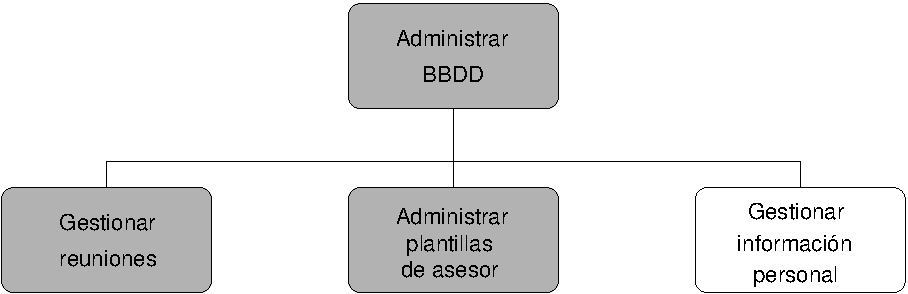
\includegraphics[]{11.Disenyo_Arquitectonico/11.2.Diagramas_Descomposicion/11.2.4.Modulo_asesores/AdministrarBBDD/Diagramas/administrar_bbdd.pdf}
      \caption{Diagrama de descomposición Administrar BBDD (módulo Asesores).}
      \label{diagramaDescomposicionAdministrarBBDD-asesores}
    \end{center}
  \end{figure}

\paragraph{}En este proceso, el usuario asesor puede crear,
consultar, modificar o borrar reuniones de la aplicación.

\paragraph{}La figura \ref{diagramaNivel4-GestionarReuniones}
muestra el nivel de abstracción 4: Gestionar reuniones.

  \begin{figure}[!ht]
    \begin{center}
      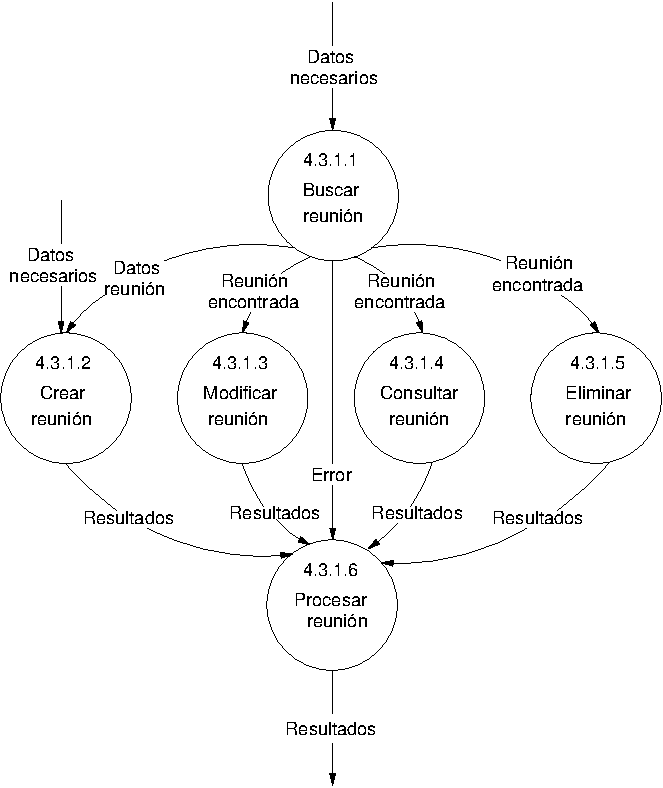
\includegraphics[]{08.Analisis_Funcional/8.2.DFDs/Niveles/Nivel4/Asesor/GestionarReuniones/Diagramas/nivel4-GestionarReuniones.pdf}
      \caption{Nivel de abstracción 4: Gestionar reuniones.}
      \label{diagramaNivel4-GestionarReuniones}
    \end{center}
  \end{figure}
